\part{Natural Deduction in QL 2}
\label{ch.qlnd2}
\addtocontents{toc}{\protect\mbox{}\protect\hrulefill\par}
\chapter{Part 26 Identity (‘=')}
\section{Part 26.1 Symbolizing Identity Statements}
\subsection{The Need for a New Connective/Predicate}

Thus far, you have everything necessary to work with QL and hopefully, apply it in your daily life, if we didn't have multiple ways of saying the same thing and we didn't obscure or leave out certain natural inferences. For example, consider this sentence:
\begin{earg}
\item[\ex{Pavel1}] Pavel owes money to everyone
\end{earg}
Let the domain be people; this will allow us to symbolize ‘everyone’ with a universal quantifier. Offering the symbolization key:
\begin{ekey}
\item[Oxy] x owes money to y
\item[p] Pavel
\end{ekey}
From this, we can symbolize sentence \ref{Pavel1} with ‘$\forall$xOpx’. But this has a (perhaps) odd consequence. It requires that Pavel owes money to every member of the domain (whatever the domain may be). The domain certainly includes Pavel. So this entails that Pavel owes money to himself. And maybe we did not want to say that. Maybe we meant to leave it open if Pavel owes money to himself, something we could have expressed more precisely by using either on of the following:
\begin{earg}
\item[\ex{Pavel2}] Pavel owes money to everyone \emph{else}
\item[\ex{Pavel3}] Pavel owes money to everyone \emph{other than Pavel}
\end{earg}
But we do not have any way for dealing with the italicised words yet. The solution is to add another symbol to QL.
\subsection{
Adding identity
}
The symbol ‘=’ will act as a two-place predicate; but, since it will have a special meaning, we shall write it a bit differently: we put it between two terms, rather than out front. (This should also be familiar; consider a mathematical equation like 1/2 = 0.5.) And the special meaning for ‘=’ is given by the fact that we always adopt the following symbolization key:
\begin{ekey}
\item[x=y] x is identical to y
\end{ekey}
This does not mean merely that the objects in question are indistinguishable, or that all of the same things are true of them. Rather, it means that the objects in question are the very same object. Also, we are using this symbol as a connective because of this very special meaning. Rather than connecting sentences, the identity symbol connects terms, names, and there are some special inference rules one can use involving this connective. To put this to use, suppose we want to symbolize this sentence:
\begin{earg}
\item[\ex{Pavel4}] Pavel is Mister Checkov.
\end{earg}
Let us add to our symbolization key:
\begin{ekey}
\item[c] Mister Checkov
\end{ekey}
Now sentence \ref{Pavel4} can be symbolized as ‘p=c’. This tells us that the names ‘p’ and ‘c’ both name the same thing. We can also now deal with sentences \ref{Pavel2} and \ref{Pavel3}. Both of these sentences can be paraphrased as ‘Everyone who is not Pavel is owed money by Pavel’. Paraphrasing some more, we get: ‘For all x, if x is not Pavel, then x is owed money by Pavel’. Now that we are armed with our new identity symbol, we can symbolize this as
\begin{center}
$\forall$x(\enot (x=p)\eif Opx)
\end{center}
You may notice that there are parentheses around ‘\enot (x=p)’, I have included those for clairity, as the identity symbol acts both as a predicate and as a connective. It is perfectly acceptable to write ‘\enot x=p’, though ahat might look a bit strange, because the symbol that comes immediately after the ‘\enot’ is a variable, rather than a predicate, but this is not a problem. We are simply negating the entire formula, ‘x=p’.
\subsection{
‘Only’ and ‘except’
}
In addition to sentences that use the word ‘else’, and ‘other than’, identity is helpful when symbolizing some sentences that contain the words ‘only’, and ‘except’. Consider:
\begin{earg}
\item[\ex{Pavel5}] Only Pavel owes money to Hikaru.
\end{earg}
Let ‘h’ name Hikaru. Plausibly, sentence \ref{Pavel5} is true if, and only if, both of the following conditions hold:
\begin{earg}
\item[\ex{Pavel6}] Pavel owes money to Hikaru.
\item[\ex{Pavel7}] No-one who is not Pavel owes money to Hikaru.
\end{earg}
Sentence \ref{Pavel7} can be symbolized by any one of:
\begin{earg}
\item[]\enot $\exists$x (\enot (x=p)\eand Oxh)
\item[]$\forall$x (\enot (x=p)\eif \enot Oxh)
\item[]$\forall$x (Oxh\eif (x=p))
\end{earg}
Thus, we can symbolize sentence \ref{Pavel5} as the conjunction of one of the above with the symbolization of \ref{Pavel6}, ‘Oph, or more compactly using ‘\eiff ’ as ‘$\forall$x(Oxh\eiff (x=p))’.
\begin{earg}
\item[\ex{Pavel8}] Everyone except Pavel owes money to Hikaru.
\end{earg}
Sentence \ref{Pavel8} can be treated similarly, although now of course Pavel does not owe Hikaru money. We can paraphrase it as ‘Everyone who is not Pavel owes Hikaru money, and Pavel does not’. Consequently, it can be symbolized as, ‘$\forall$x (\enot (x=p)\eif  Oxh)\eand \enot Oph’, or more concisely, ‘$\forall$x(\enot (x=p)\eiff Oxh)’. Other locutions akin to ‘except’ such as ‘but’ or ‘besides’ (as used in ‘no-one but Pavel’ or ‘someone besides Hikaru’) can be treated in similar ways.

The above treatment of so-called “exceptives” is not uncontentious. Some linguists think that sentence \ref{Pavel8} does not entail that Pavel doesn’t owe Hikaru money, and so the symbolization should just be ‘$\forall$x (\enot (x=p)\eif Oxh)’. There are also uses of ‘except’ that clearly do not have that entailment, especially in mathematical writing. For instance, you may read in a calculus textbook that “the function f is defined everywhere except possibly at a”. That means only that for every point x other than a, f is defined at x. It is not required that f is undefined at a; it’s left open whether f is or is not defined at a.

\subsection{There are at least\ldots}

We can also use identity to say how many things there are of a particular kind. For example, consider these sentences:
\begin{earg}
\item[\ex{apple1}] There is at least one apple
\item[\ex{apple2}] There are at least two apples
\item[\ex{apple3}] There are at least three apples
\end{earg}
We will use the symbolization key:
\begin{ekey}
\item[Ax] x is an apple
\end{ekey}
Sentence \ref{apple1} does not require identity. It can be adequately symbolized by ‘$\exists$x Ax’: There is an apple; perhaps many, but at least one.

It might be tempting to also symbolize sentence \ref{apple2} without identity. Yet consider the sentence ‘$\exists$x$\exists$y(Ax\eand Ay)’. Roughly, this says that there is some apple x in the domain and some apple y in the domain. Since nothing precludes these from being one and the same apple, this would be true even if there were only one apple. In order to make sure that we are dealing with different apples, we need an identity predicate. Sentence \ref{apple2} needs to say that the two apples that exist are not identical, so it can be symbolized by ‘$\exists$x$\exists$y( (Ax\eand Ay)\eand \enot (x=y))’.

Sentence \ref{apple3} requires talking about three different apples. Now we need three existential quantifiers, and we need to make sure that each will pick out something different:
\begin{center}
$\exists$x$\exists$y$\exists$z[((Ax\eand Ay)\eand Az)\eand ((\enot (x=y)\eand \enot (y=z))\eand \enot (x=z))]
\end{center}
Note that it is not enough to use ‘\enot (x=y)\eand \enot (y=z)’ to symbolize ‘x, y, and z are all different.’ For that would be true if x and y were different, but x=z. In general, to say that x1,\ldots, xn are all different, we must have a conjunction of \enot (xi=xj) for every different pair i and j .
\subsection{
There are at most\ldots
}
Now consider these sentences:
\begin{earg}
\item[\ex{appleonly1}] There is at most one apple
\item[\ex{appleonly2}] There are at most two apples
\end{earg}
Sentence \ref{appleonly1} can be paraphrased as, ‘It is not the case that there are at least two apples’. This is just the negation of sentence \ref{apple2}:
\begin{center}
\enot $\exists$x$\exists$y[(Ax \eand Ay)\eand \enot (x=y)]
\end{center}
But sentence \ref{appleonly1} can also be approached in another way. It means that if you pick out an object and it’s an apple, and then you pick out an object and it’s also an apple, you must have picked out the same object both times. With this in mind, it can be symbolized by
\begin{center}
$\forall$x$\forall$y[Ax\eand Ay)\eif (x=y)]
\end{center}
The two sentences will turn out to be logically equivalent.

Similarly, sentence \ref{appleonly2} can be approached in two equivalent ways. It can be paraphrased as, ‘It is not the case that there are three or more distinct apples’, so we can offer:
\begin{center}
\enot $\exists$x$\exists$y$\exists$z[((Ax\eand Ay)\eand Az)\eand ((\enot (x=y)\eand \enot (x=z))\eand \enot (y=z))]
\end{center}
Alternatively we can read it as saying that if you pick out an apple, and an apple, and an apple, then you will have picked out (at least) one of these objects more than once. Thus:
\begin{center}
$\forall$x$\forall$y$\forall$z((Ax\eand Ay)\eand Az)\eif (((x=y)\eor (x=z))\eor (y=z))]
\end{center}
\subsection{There are exactly\ldots}

We can now consider precise of numerical quantity, like:
\begin{earg}
\item[\ex{appleexact1}]There is exactly one apple.
\item[\ex{appleexact2}]There are exactly two apples.
\item[\ex{appleexact3}]There are exactly three apples.
\end{earg}
Sentence \ref{appleexact1} can be paraphrased as, ‘There is at least one apple and there is at most one apple’. This is just the conjunction of sentence \ref{apple1} and sentence \ref{appleonly1}. So we can offer:
\begin{center}
$\exists$xAx\eand $\forall$x$\forall$y[(Ax\eand Ay)\eif (x=y)]
\end{center}
But it is perhaps more straightforward to paraphrase sentence \ref{appleexact1} as, ‘There is a thing x which is an apple, and everything which is an apple is just x itself’. Thought of in this way, we offer:
\begin{center}
$\exists$x[Ax\eand $\forall$y(Ay\eif (x=y))]
\end{center}
Similarly, sentence \ref{appleexact2} may be paraphrased as, ‘There are at least two apples, and there are at most two apples’. Thus we could offer:
\begin{center}
$\exists$x$\exists$y((Ax\eand Ay)\eand \enot (x=y)\eand $\forall$x$\forall$y$\forall$z[((Ax\eand Ay)\eand Az)\eif (((x=y)\eor (x=y))\eor (y=z))]
\end{center}
More efficiently, though, we can paraphrase it as ‘There are at least two different apples, and every apple is one of those two apples’. Then we offer:
\begin{center}
$\exists$x$\exists$y[︁((Ax\eand Ay)\eand \enot (x=y))\eand $\forall$z(Az\eif ((x=z)\eor (y=z)))]︁
\end{center}
Finally, consider these sentences:
\begin{earg}
\item[\ex{twothings}] There are exactly two things.
\item[\ex{twoobjects}] There are exactly two objects.
\end{earg}
It might be tempting to add a predicate to our symbolization key, to symbolize the English predicate ‘x is a thing’ or ‘x is an object’, but this is unnecessary. Words like ‘thing’ and ‘object’ do not sort wheat from chaff: they apply trivially to everything, which is to say, they apply trivially to every thing. So we can symbolize either sentence with either of the following:
\begin{center}
$\exists$x$\exists$y\enot (x=y)\eand \enot $\exists$x$\exists$y$\exists$z((\enot (x=y)\eand \enot (y=z))\eand \enot (x=z))\\
$\exists$x$\exists$y[︁\enot (x=y)\eand $\forall$z((x=z)\eor (y=z))]
\end{center}
\section{Part 26.2 The Semantics and Rules for Identity}
\subsection{Semantics for identity}

Identity is a special predicate of QL as it can also function as a connective. Because of this, we write it a bit differently than other two-place predicates: ‘x=y’ instead of ‘Ixy’, or something like that. More important, though, its interpretation is fixed, once and for all. Much like how regardless of the interpretation, the connectives always behave the same way (given their inputs), identity will always mean and behave the same way regardless of interpretation.

If two names refer to the same object, then swapping one name for another will not change the truth value of any sentence. So, in particular, if ‘a’ and ‘b’ name the same object, then all of the following will be true:
\begin{earg}
\item[]Aa\eiff Ab
\item[]Ba\eiff Bb
\item[]Raa\eiff Rbb
\item[]Raa\eiff Rab
\item[]Rca\eiff Rcb
\item[]$\forall$ xRxa\eiff $\forall$ xRxb
\end{earg}
Some philosophers have believed the reverse of this claim. That is, they have believed that when exactly the same sentences (not containing ‘=’) are true of a and b, then a and b are the very same object. This is a highly controversial philosophical claim— sometimes called the identity of indiscernibles —and our logic will not subscribe to it; we allow that exactly the same things might be true of two distinct objects. To bring this out, consider the following interpretation:
\begin{ekey}
\item[domain] P.D. Magnus, Tim Button
\item[a] P.D. Magnus
\item[b] Tim Button
\item[\textbullet] For every primitive predicate we care to consider, that predicate is true of nothing.
\end{ekey}
Suppose ‘A’ is a one-place predicate; then ‘Aa’ is false and ‘Ab’ is false, so ‘Aa\eiff Ab’ is true. Similarly, if ‘R’ is a two-place predicate, then ‘Raa’ is false and ‘Rab’ is false, so that ‘Raa\eiff Rab’ is true. And so it goes: every atomic sentence not involving ‘=’ is false, so every biconditional linking such sentences is true. For all that, Tim Button and P.D. Magnus are two distinct people, not one and the same!

\subsection{Rules for identity}

Above, we mentioned the philosophically contentious thesis of the identity of indiscernibles. This is the claim that objects which are indiscernible in every way are, in fact, identical to each other. It was also mentioned that we will not subscribe to this thesis. It follows that, no matter how much you learn about two objects, we cannot prove that they are identical. That is unless, of course, you learn that the two objects are, in fact, identical, but then the proof will hardly be very illuminating.

The general point, though, is that no sentences which do not already contain the identity predicate could justify an inference to ‘a=b’. So our identity introduction rule cannot allow us to infer to an identity claim containing two different names.

However, every object is identical to itself. No premises, then, are required in order to conclude that something is identical to itself. So this will be the identity introduction rule:
\factoidbox{\begin{fitchproof}
\have[m]{a}{c=c}\ii{}	
\end{fitchproof}}
Notice that this rule does not require referring to any prior lines of the proof. For any name c, you can write c = c on any point, with only the =I rule as justification.

Our elimination rule is more fun. If you have established ‘a=b’, then anything that is true of the object named by ‘a’ must also be true of the object named by ‘b’. For any sentence with ‘a’ in it, you can replace some or all of the occurrences of ‘a’ with ‘b’ and produce an equivalent sentence. For example, from ‘Raa’ and ‘a=b’, you are justified in inferring ‘Rab, ‘Rba’ or ‘Rbb’. More generally:
\factoidbox{\begin{fitchproof}
\have{m}{a=b}
\have{n}{A\ldots a\ldots a\ldots}
\have{p}{A\ldots b\ldots a\ldots}\ie{m,n}	
\end{fitchproof}}
The notation here is as for $\exists$ I. So A\ldots a\ldots a\ldots  is a formula containing the name a, and A\ldots b\ldots a\ldots  is a formula obtained by replacing one or more instances of the name a with the name b. Lines m and n can occur in either order, and do not need to be adjacent, but we always cite the statement of identity first. Symmetrically, we allow:
\begin{fitchproof}
\have{m}{a=b}
\have{n}{A\ldots a\ldots a\ldots }
\have{p}{A\ldots a\ldots b\ldots }\ie{m,n}	
\end{fitchproof}

This rule is sometimes called Leibniz’s Law, after Gottfried Leibniz. To see the rules in action, we will prove some quick results. First, we will prove that identity is symmetric:
\begin{fitchproof}
\open
\hypo{1}{a=b}
\have{2}{a=a}\ii{}	
\have{3}{b=a}\ie{1,2}	
\close
\have{4}{(a=b)\eif (b=a)}\ci{1-3}	
\have{5}{\forall y((a=y)\eif (y=a))}\Ai{4}
\have{6}{\forall x\forall y((x=y)\eif (y=x))}\Ai{5}
\end{fitchproof}
We obtain line 3 by replacing one instance of ‘a’ in line 2 with an instance of ‘b’; this is justified given ‘a=b’. Second, we will prove that identity is transitive:
\begin{fitchproof}
\open
\hypo{1}{(a=b)\eand (b=c)}			
\have{2}{a=b}\ae{1}
\have{3}{b=c}\ae{1}
\have{4}{a=c}\ie{2,3}
\close
\have{5}{((a=b)\eand (b=c))\eif (a=c)}\ci{1-4}
\have{6}{\forall z(((a=b)\eand (b=z))\eif (a=z))}\Ai{5}
\have{7}{\forall y\forall z(((a=y)\eand (y=z))\eif (a=z))}\Ai{6}
\have{8}{\forall x\forall y\forall z(((a=y)\eand (y=z))\eif (a=z))}\Ai{7}
\end{fitchproof}
We obtain line 4 by replacing ‘b’ in line 3 with ‘a’; this is justified given ‘a = b’.

\leibniz
\practiceproblems
\problempart
\label{pr.TorF3}
Consider the following interpretation, represented as a model:	
\begin{center}
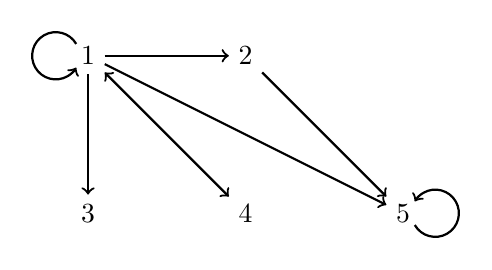
\begin{tikzpicture}
\node (atom1) at (0,2) {$1$};
\node (atom2) at (2,2) {$2$};
\node (atom4) at (0,0) {$3$};
\node (atom5) at (2,0) {$4$};
\node (atom6) at (4,0) {$5$};
\draw[->, thick] (atom1)+(-0.15,0.15) arc (-330:-30:.3); 
\draw[->, thick] (atom6)+(0.15,-0.15) arc (-150:150:.3); 
\draw[->, thick] (atom1) -- (atom2);
\draw[->, thick] (atom1) -- (atom4);
\draw[<->, thick] (atom1) -- (atom5);
\draw[->, thick] (atom1) -- (atom6);
\draw[->, thick] (atom2) -- (atom6);
\end{tikzpicture}
\end{center}
Determine whether each of the following sentences is true or false in that interpretation:
\begin{enumerate}
\item $\exists x\, \atom{R}{xx}$
\item $\forall x\, \atom{R}{xx}$
\item $\exists x \forall y\, \atom{R}{xy}$
\item $\exists x \forall y\, \atom{R}{yx}$
\item $\forall x \forall y \forall z ((\atom{R}{xy} \eand \atom{R}{yz}) \eif \atom{R}{xz})$
\item $\forall x \forall y \forall z ((\atom{R}{xy} \eand \atom{R}{xz}) \eif \atom{R}{yz})$
\item $\exists x \forall y\, \enot \atom{R}{xy}$
\item $\forall x(\exists y\, \atom{R}{xy} \eif \exists y\, \atom{R}{yx})$
\item $\exists x \exists y (\enot x = y \eand \atom{R}{x,y} \eand \atom{R}{yx})$
\item $\exists x \forall y(\atom{R}{xy} \eiff x = y)$
\item $\exists x \forall y(\atom{R}{yx} \eiff x = y)$
\item $\exists x \exists y(\enot x = y \eand \atom{R}{xy} \eand \forall z(\atom{R}{zx} \eiff y = z))$
\end{enumerate}
\problempart
Determine whether each of the following is valid or invalid, construct a proof if valid:
\begin{enumerate}
\item $\therefore \exists x (x = h \eand x = i)$
\item $\forall x(\atom{D}{x} \eif \exists y\, \atom{T}{yx}) \therefore \exists y \exists z\ \enot y= z$
\item $\enot \atom{R}{aa}$, $\forall x (x=a \eor \atom{R}{xa})$
\item $\forall x\forall y\forall z[(x=y \eor y=z )\eor x=z]$, $\exists x\exists y\ \enot x= y$
\item $\exists x\exists y((\atom{Z}{x} \eand \atom{Z}{y} )\eand x=y)$, $\enot \atom{Z}{d}$, $d=e$
\end{enumerate}



\chapter{Part 27 Equivalency Rules in QL}
\section{Part 27.1 The Equivalency Rules in PL are in QL}
As was previously mentioned, QL is an extension of PL. This means that not only do you have access to all of the inferences rules in PL but you also have access to all of the equivalency rules as well. Just like in PL, these rules can be applied to the main operator of a sentence (the entire sentence) or to just a part of it. it is worth remembering that equivalency rules are different from inference rules. Inference rules can only be done on the main operator and typically require two, or more, lines for the citation. Equivalency rules are basically when you are saying the same thing as before but in a different way (as I have mentioned). 

All that said, in QL, you can use Double Negation (DN), Commutativity (Comm), Material Conditional (MC), Biconditional Exchange (\eiff ex), DeMorgan's (DeM), and Tautology (TAUT). Below is a basic overview (refresher) of these rules and some examples of how they can be helpful in QL.

\subsection{DN and Comm}

Very often in QL, the main operator for a sentence will not be a connective like we had in PL, rather, it will be a quantifier. This means that when you are working with a complex sentence, you will need to use these equivalency rules. As with PL, Double Negation is the simplest; but you need to be careful that the two negations are right next to each other, nothing (not even a bracket) is between them. Double Negation is especially useful with the Quantifier Negation rule (next page). As a refresher, the rule looks like this: 
\factoidbox{
\enot \enot \metav{A} $\Leftrightarrow$ \metav{A}
}
'A' could be a simple or complex sentence and A could be the entire sentence or just a part. The major thing to remember is that the two negations are right beside each other. For example, this is not correct:
\begin{fitchproof}
\hypo{1}{\enot \exists x\enot Px}
\have{2}{\exists xPx}\by{naughty attempt to use DN}{1}
\end{fitchproof}
While it is true that, in this case, it is valid, there is a few missing steps of reasoning which you need to be aware of (through the Quantifier Negation rule). For a more egregious example of this sort of error, take a look at this: 
\begin{fitchproof}
\hypo{1}{\forall x\enot (\enot Px\eif Qx)}
\have{2}{\forall x(Px\eif Qx)}\by{naughty attempt to use DN}{1}	
\end{fitchproof}

The first line (1) is saying, roughly, that for anything, it's not the case that if it's not P, then it's Q or, in other words, everything is P and Q. The second line says something very different; namely, for anything, if it's P, then it's Q. 

Commutativity is another surprisingly useful rule in QL but it has it's caveats as well. To remind you, here are the different ways Comm can be used: 
\factoidbox{
(\metav{A}\eand \metav{B}) $\Leftrightarrow$ (\metav{B}\eand \metav{A})\\
(\metav{A}\eor \metav{B}) $\Leftrightarrow$ (\metav{B}\eor \metav{A})\\
(\metav{A}\eiff \metav{B}) $\Leftrightarrow$ (\metav{B}\eiff \metav{A})
}
When dealing with a sentence where the main operator is a conjunction, disjunction, or biconditional (those which are symmetric), you can flip the order without any worries. There is, however, one key, relatively common, error you need to be aware of:
\begin{fitchproof}
\hypo{1}{\forall x\exists yPxy}
\have{2}{\exists y\forall xPxy}\by{naughty attempt to use COMM}{1}	
\end{fitchproof}
 As you may recall, this is not a valid inference and these statements are not equivalent. The scope of the operators matters. You can avoid this sort of reasoning by being mindful of the fact that Comm only works in cases like those listed above. 

\subsection{MC and \eiff ex}

Material Conditional is very useful when dealing with negated conditionals (one of my favorite cases), but it is also useful when trying to work with mismatched consequents and antecedents.  Here are the cases where it can be used: 
\factoidbox{
(\metav{A}\eif \metav{B}) $\Leftrightarrow$ (\enot \metav{A}\eor \metav{B})\\
(\metav{A}\eor \metav{B}) $\Leftrightarrow$ (\enot \metav{A}\eif \metav{B})
}
This allows us to move between conditionals and disjunctions. There are not very many common errors or confusions with this one, but it is essential that you remember to tack-on the negation as required, even if there is one already there for example, in a case like this:
\begin{center}
(\enot A\eif B) \therefore  (\enot \enot A\eor B)
\end{center}
If your goal is actually A\eor B, then you can simply do a DN as an `additional' step. If you get comfortable skipping this DN step, you will be more prone to errors in your thinking in the future. 

Remember that \eiff ex is the one way we have to work with biconditionals. We need to use this step to derive things using biconditionals. Since biconditionals are conjoined conditionals, the rule looks like this: 
\factoidbox{
[(A\eif B)\eand (B\eif A)] $\Leftrightarrow$ (A\eiff B)
}
There are scant few errors made using this rule, but don't get too relaxed about it. For an example of how we can use this in QL, let's try this argument: 
\begin{center}
$\forall$ x(Px\eiff Qx) \therefore  $\forall$ x(Px\eif Qx)
\end{center}
This argument is valid, just like the QL version, here is the proof:
\begin{fitchproof}
\hypo{1}{\forall x(Px\eiff Qx)}
\have{2}{\forall x[(Px\eif Qx)\eand (Qx\eif Px)]}\by{\eiff ex}{1}
\have{3}{(Pa\eif Qa)\eand (Qa\eif Pa)}\Ae{2}
\have{4}{Pa\eif Qa}\ae{3}
\have{5}{\forall x(Px\eif Qx)}\Ai{4}
\end{fitchproof}
\subsection{DeM and TAUT}

DeMorgan's Law(s) are some of my personal favorites in Logic, and they are shockingly useful. As a reminder, DeMorgan's Law(s) essentially say that `neither X nor Y' means the same thing as `not-X and not-Y'. Similarly, they say that `not-X or not-Y' means the same as `not both X and Y'. This is symbolized like so: 
\factoidbox{
\enot (\metav{A}\eor \metav{B}) $\Leftrightarrow$ (\enot \metav{A}\eand \enot \metav{B})\\
\enot (\metav{A}\eand \metav{B}) $\Leftrightarrow$ (\enot \metav{A}\eor \enot \metav{B})
}
Like with Double Negation, it is good to remember that there can't be anything between the negation and the sentence with one of these main operators. For example, here is a naughty attempt: 
\begin{fitchproof}
\hypo{1}{\enot \forall x(Px\eor Qx)}
\have{2}{\forall x(\enot Px\eand \enot Qx)}\by{naughty attempt to use DeM}{1}	
\end{fitchproof}
The first line is saying, essentially, that something (at least one thing) is neither P nor Q while the second line is saying that everything is neither P nor Q. Those are very different statements. 

Tautology, as an equivalency rule not a kind of statement, comes in handy more often that you would think. We normally gloss over this in our reasoning but it is worthwhile to remember that errors happen when we aren't paying attention. TAUT works like this:
\factoidbox{
(\metav{A}\eor \metav{A}) $\Leftrightarrow$ (\metav{A})\\
(\metav{A}\eand \metav{A}) $\Leftrightarrow$ (\metav{A})
}
To see this equivalency rule at work in QL, take a look at this argument:
\begin{center}
$\forall$ x(Px\eif (Qx\eand Qx)),$\forall$ x(Qx\eif \enot Px) \therefore  $\forall$ x\enot Px
\end{center}
And here is the proof:
\begin{fitchproof}
\hypo{1}{\forall x(Px\eif (Qx\eand Qx))}
\hypo{2}{\forall x(Qx\eif \enot Px)}
\have{3}{\forall x(Px\eif Qx)}\by{TAUT}{1}
\have{4}{Pa\eif Qa}\Ae{3}
\have{5}{Qa\eif \enot Pa	}\Ae{2}
\have{6}{Pa\eif \enot Pa}\hs{4,5}
\have{7}{\enot Pa\eor \enot Pa}\mc{6}
\have{8}{\enot Pa}\by{TAUT}{7}
\have{9}{\forall x\enot Px}\Ai{8}	
\end{fitchproof}

We conclude here with everything isn't P. 
\section{Part 27.2 Change of Quantifier (Quantifier Negation)}
When we are symbolizing statements into QL, it should be noted that \enot $\forall$ x\enot Ax is logically equivalent to $\exists$ xAx and this makes sense. For example, if I say "it's not the case that everything isn't purple", this is just a long-winded way of saying that "something is purple". Similarly, \enot $\exists$ x\enot Ax is equivalent to $\forall$ xAx, and this too makes sense; if I say "it's not the case that someone isn't happy", this is, again, a long winded way of saying that "everyone is happy." In QL, these are actually provably equivalent, but it is a rather gruesome, involved proof. If you would like, for an added exersize, try to prove the following:
\begin{earg}
\item[]\enot $\forall$ x\enot Ax \therefore  $\exists$ xAx
\item[]\enot $\exists$ x\enot Ax \therefore  $\forall$ xAx
\item[]$\forall$ x\enot Ax \therefore  \enot $\exists$ xAx
\item[]$\exists$ x\enot Ax \therefore  \enot $\forall$ xAx
\end{earg}
Since the proofs for these are very involved and it would become very tiresome to need to run through the proofs every time you wanted to switch between these (when they are logically equivalent), we have given you a simple rule of equivalence, called Quantifier Negation (QN):
\factoidbox{
$\exists$ x\enot Ax $\Leftrightarrow$ \enot $\forall$ xAx\\
$\forall$ x\enot Ax $\Leftrightarrow$ \enot $\exists$ xAx
}
As a reminder, the `$\Leftrightarrow$' means that you can switch between these (the rule goes both ways) and the rule is an equivalency rule, meaning that it can be used in anywhere, even when it is not the main operator. One way to metaphorically think about this is that the negation is a snake and when it climbs over the quantifier, the snake flips it, from $\exists$  to $\forall$  or from $\forall$  to $\exists$  and then falls asleep on the other side. To see this in action, let's return to my favorite example for equivalency rules, now in QL rather than PL:
\begin{center}
\enot $\forall$ x(Ux\eif \enot Hx) \therefore  $\exists$ x(Ux\eand Hx)
\end{center}
In principle, we could read this as "it's not the case that for any x you pick, if x is a unicorn, then x doesn't have a horn. Therefore, there is an x such that x is a unicorn and x has a horn.". This might seem rather funny, but it is a perfectly valid argument and one which we can prove using all of the equivalency rules at our disposal:
\begin{fitchproof}
\hypo{1}{\enot \forall x(Ux\eif \enot Hx)}
\have{2}{ \enot \forall x(\enot Ux\eor \enot Hx)} \by{MC}{1}
\have{3}{\exists x\enot (\enot Ux\eor \enot Hx)}\by{QN}{2}
\have{4}{\exists x(\enot \enot Ux\eand \enot \enot Hx)}\by{DeM}{3}
\have{5}{\exists x(Ux\eand \enot \enot Hx)}\by{DN}{4}
\have{6}{\exists x(Ux\eand Hx)}\by{DN}{5}	
\end{fitchproof}
You might now be thinking "what about `\enot $\forall$ x\enot' and `\enot $\exists$ x\enot`? How can I use those?" Well, you need to remember that DN is allowed in QL, so, when you have something like \enot $\forall$ x\enot Px and you want $\exists$ xPx, just follow these steps, so something like them:
\begin{fitchproof}
\hypo{1}{\enot \forall x\enot Px}
\have{2}{\exists x\enot \enot Px}\by{QN}{1}
\have{3}{\exists xPx}\by{DN}{2}	
\end{fitchproof}
These steps can be done on something contained in a sentence or on the main operator. They are both equivalency rules, after all. Similarly, if you want to go from \enot $\exists$ x\enot Px to $\forall$ xPx, you need to follow similar steps:
\begin{fitchproof}
\hypo{1}{\enot \exists x\enot Px}
\have{2}{\forall x\enot \enot Px}\by{QN}{1}
\have{3}{\forall xPx}\by{DN}{2}	
\end{fitchproof}

Personally, I prefer having the negation move inward in the sentence when dealing with cases like this, but this is exclusively a matter of preference, there is nothing against doing these steps like this: 
\begin{fitchproof}
\hypo{1}{\enot \forall x\enot Px}
\have{2}{\enot \enot \exists xPx}\by{QN}{1}
\have{3}{\exists xPx}\by{DN}{2}	
\end{fitchproof}

Or like this:
\begin{fitchproof}
\hypo{1}{\enot \exists x\enot Px}
\have{2}{\enot \enot \forall xPx}\by{QN}{1}
\have{3}{\forall xPx}\by{DN}{2}	
\end{fitchproof}

\barcan

\practiceproblems
\problempart
Use the strategies to find proofs for each of the following arguments and theorems:
\begin{enumerate}
\item $A \eif \forall x\,\atom{B}{x} \therefore \forall x(A \eif \atom{B}{x})$
\item $\exists x(A \eif \atom{B}{x}) \therefore A \eif \exists x\, \atom{B}{x}$
\item $\forall x(\atom{A}{x} \eand \atom{B}{x}) \eiff (\forall x\,\atom{A}{x} \eand \forall x\,\atom{B}{x})$
\item $\exists x(\atom{A}{x} \eor \atom{B}{x}) \eiff (\exists x\,\atom{A}{x} \eor \exists x\,\atom{B}{x})$
\item $A \eor \forall x\,\atom{B}{x}) \therefore \forall x(A \eor \atom{B}{x})$
\item $\forall x(\atom{A}{x} \eif B) \therefore \exists x\,\atom{A}{x} \eif B$
\item $\exists x(\atom{A}{x} \eif B) \therefore \forall x\,\atom{A}{x} \eif B$
\item $\forall x(\atom{A}{x} \eif \exists y\,\atom{A}{y})$
\end{enumerate}
Use only the basic rules of QL in addition to the basic quantifier rules.

\problempart
Use the strategies to find proofs for each of the following arguments and theorems:
\begin{enumerate}
\item $\forall x\,\atom{R}{xx} \therefore \forall x\,\exists y\,\atom{R}{xy}$
\item $\forall x\,\forall y\,\forall z[(\atom{R}{xy} \eand \atom{R}{y,z}) \eif \atom{R}{xz}]$ \\
$\therefore \forall x\,\forall y[\atom{R}{xy} \eif \forall z(\atom{R}{yz} \eif \atom{R}{xz})]$
\item $\forall x\,\forall y\,\forall z[(\atom{R}{xy} \eand \atom{R}{yz}) \eif \atom{R}{xz}],$\\ $\forall x\,\forall y(\atom{R}{xy} \eif \atom{R}{yx})$ \\ $\therefore \forall x\,\forall y\,\forall z[(\atom{R}{xy} \eand \atom{R}{xz}) \eif \atom{R}{yz}]$
\item $\forall x\,\forall y(\atom{R}{xy} \eif \atom{R}{yx})$ \\$\therefore \forall x\,\forall y\,\forall z[(\atom{R}{xy} \eand \atom{R}{xz}) \eif \exists u(\atom{R}{yu} \eand \atom{R}{zu})]$
\item $\enot \exists x\,\forall y (\atom{A}{xy} \eiff \lnot\atom{A}{yy})$
\end{enumerate}

\problempart
Use the strategies to find proofs for each of the following arguments and theorems:
\begin{enumerate}
\item $\forall x\,\atom{A}{x} \eif B \therefore \exists x(\atom{A}{x} \eif B)$
\item $A \eif \exists x\, \atom{B}{x} \therefore \exists x(A \eif \atom{B}{x})$
\item $\forall x(A \eor \atom{B}{x}) \therefore A \eor \forall x\,\atom{B}{x})$
\item $\exists x(\atom{A}{x} \eif \forall y\,\atom{A}{y})$
\item $\exists x(\exists y\,\atom{A}{y} \eif \atom{A}{x})$
\end{enumerate}
